%# -*- coding: utf-8-unix -*-
%%==================================================
%% chapter05.tex
%%==================================================

%\bibliographystyle{sjtu2}%[此处用于每章都生产参考文献]
\chapter{系统架构与开发实现}
\label{chap:design_and_implement}
本系统基于敏捷开发、响应式设计、Flux架构模式等理论指导,在简洁且充分的需求分析的基础之上,使用全栈JS技术和各类高效的开发工具开始了系统设计与开发。三个模块使用的各类理论、技术和工具互有重叠:
\begin{itemize}
  \item 在开发模式方面,都是使用的敏捷开发,频繁部署新版本的同时不断地根据需求和反馈迭代开发。
  \item 在UI设计和页面布局方面,都使用了Flex布局和google的Material design,程序员能够方便地控制页面布局,同时页面也简洁美观富有质感。
  \item 在API设计方面,各有一套RESTful风格的API让APP能够方便地增删改查各类资源,同时WebSocket的使用让APP能够及时地获得数据更新。
  \item 在权限校验方面,在Oauth和JWT的帮助下,用户能够安全、方便地访问我们的系统,将来系统也很容易加上单点认证系统或者接入其他第三方平台。
  \item 在版本控制和代码风格方面,都使用了Git和Git flow来控制版本和发布,使用了JSCS、stylelint、pre-commit和代码审查来保证代码风格的一致。
  \item 在测试方面,都选择了Karma+Mocha+Chai+Sinon的技术栈,加上Solano CI来持续集成和自动部署。
\end{itemize}
\section{版本管理模块}
本模块使用基于比较成熟的MEAN技术栈,即MongoDB+ExpressJS+AngularJS+NodeJS。本模块比较特殊的一点在于使用了代码生成器,本文作者也是这个项目的主要代码贡献者之一。另外本模块在页面布局方面额外使用了响应式设计来使得页面能够适应所有大于平板的屏幕宽度,使用了gulp作为构建工具,使用jshint来检查语法,前后端分别使用了Atom和Webstorm来编辑源代码。
\subsection{API}
本模块使用RESTful风格的API,包含新建、删除、修改、列表查询和单一查询五种API,围绕Mongoose的数据模型来进行增删改查等业务,同时使用WebSocket在保存和删除的同时发送消息给前端,让前端及时获悉改动。如图4-1所示,这是传感器API完整的目录结构,其中包含controller(业务逻辑控制器)、model(Mongoose数据模型)、params(查询参数)和socket(WebSocket事件注册)以及两个测试文件。
\begin{figure}[H]
 \centering
 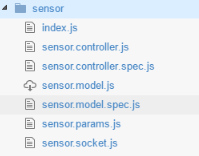
\includegraphics[width=0.4\textwidth]{sensor_api_files.png}
 \bicaption[fig:sensor_api_files]{传感器API目录结构}{传感器API目录结构}{Fig}{Directory of Sensor's API}
\end{figure}
这里的业务逻辑控制器里面其实没有真正的增删改查逻辑,因为增删改查等操作是每个资源的API都应该有的,所以它们被泛化到了控制器的基类CrudController中。如代码4-1所示,CrudController是一个构造函数,接收一个模型(model)作为参数,所以不同的业务逻辑控制器可以传入各自的model就可以使用基类的增删改查函数来注册API了。
\begin{lstlisting}[language={JavaScript}, caption={传感器API定义}]
/* in crud.controller.js */
function CrudController(model) {
  // set the model instance to work on
  this.model = model;
}
/* in sensor.controller.js */
function SensorController(router) {
  // call super constructor
  CrudController.call(this, Sensor,  router);
}
/* in sensor/index.js */
// register sensor routes
router.route('/')
  .get(controller.index)
  .post(controller.create);

router.route('/' + controller.paramString)
  .get(controller.show)
  .delete(controller.destroy)
  .put(controller.update)
  .patch(controller.update);
\end{lstlisting}

如代码4-2所示,本模块在socket文件中给传感器模型的保存和删除操作添加了钩子(hook),一旦保存或删除则用WebSocket发送'sensor:save'或'sensor:remove'的消息并附上保存完或删除前的对象,用以通知前端。
\begin{lstlisting}[language={JavaScript}, caption={Sensor的Mongoose模型}]
/* in sensor.socket.js */
function registerSensorSockets(socket) {
  Sensor.schema.post('save', function (doc) {
    onSave(socket, doc);
  });

  Sensor.schema.post('remove', function (doc) {
    onRemove(socket, doc);
  });
}

function onSave(socket, doc, cb) {
  socket.emit('sensor:save', doc);
}

function onRemove(socket, doc, cb) {
  socket.emit('sensor:remove', doc);
}
\end{lstlisting}

如代码4-3所示,传感器的数据模型通过一个可嵌套的对象来定义。
\begin{lstlisting}[language={JavaScript}, caption={传感器的Mongoose数据模型}]
var SensorDefinition = {
  name: {type: String, required: true},
  hardwareVersion: {type: ObjectId, ref: 'HardwareVersion'},
  firmwareVersion: {type: ObjectId, ref: 'FirmwareVersion'},
  componentBatches: {
    body: {type: ObjectId, ref: 'ComponentBatch'},
    pcb: {type: ObjectId, ref: 'ComponentBatch'},
    photodiode: {type: ObjectId, ref: 'ComponentBatch'},
    laser: {type: ObjectId, ref: 'ComponentBatch'},
    fan: {type: ObjectId, ref: 'ComponentBatch'},
  },
  threshold: {type: Number, required: true},
  noiseLevel: {type: Number, required: true},
  calibrations: {
    mass: Number,
    number: Number
  },
  applicationType: String,
  info: String,
  active: Boolean
};
\end{lstlisting}
\subsection{API路由}
在AngularJS中一个页面由四份代码渲染而成,分别是HTML代码、样式代码、控制器代码和路由器(router)代码。在本模块中把这四份代码分别写在一个文件中,合起来的目录结构叫做一个路由(route);把一套创建、列表、详细和编辑的页面叫做API路由(apiroute),因为它是一套与增删改查API相对应的路由的集合。一个API路由中除了增删改查的基本路由,还有两个抽象路由list和sensor,因为它们的控制器里面几乎没有业务逻辑,HTML代码也不包含任何实际有意义的内容,只是在路由器层面组织起这个结构,特殊的是在这里list路由作为一个插入点对传感器的WebSocket进行了监听,在列表中及时地更新被创建、修改或删除的内容。一个API路由的额外包含一个资源服务(resource service),提供与API交互的所有增删改查函数。

如图4-2所示,这是传感器API路由完整的目录结构,其中sensor.html、sensor.scss、sensor.contoller.js和sensor.js文件分别对应上述四份代码,main、create、detail、edit和items都分别是一个完整的路由,sensor.service.js就是用来定义传感器的资源服务的文件。在这里main路由是create路由和list路由的入口,不作过多介绍。
\begin{figure}[H]
 \centering
 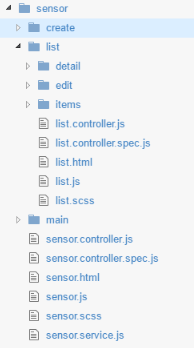
\includegraphics[width=0.4\textwidth]{sensor_files.png}
 \bicaption[fig:sensor_files]{传感器API路由目录结构}{传感器API路由目录结构}{Fig}{Directory of Sensor's apiroute}
\end{figure}

这里以用户页面为例,展示API路由的全貌,如图4-3所示,这套设计让create页面以一个弹窗(modal)的形式浮在list上方;如图4-4和4-5所示,detail页面和edit页面从list右方弹出;如图4-6所示,一旦有数据更新,会有toastr\footnote{一个专门做窗口提示的JavaScript库}窗口提示。
\begin{figure}[H]
 \centering
 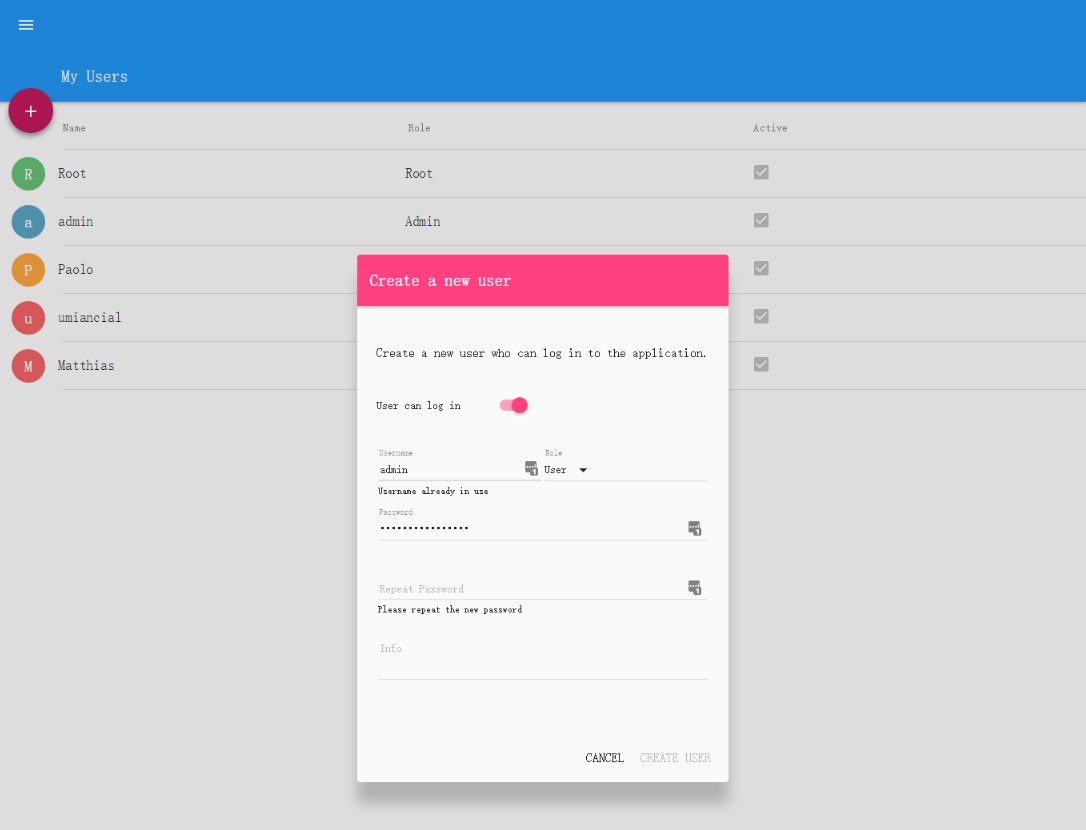
\includegraphics[width=\textwidth]{user_create.png}
 \bicaption[fig:user_create]{用户创建页面}{用户创建页面}{Fig}{Create page of User}
\end{figure}
\begin{figure}[H]
 \centering
 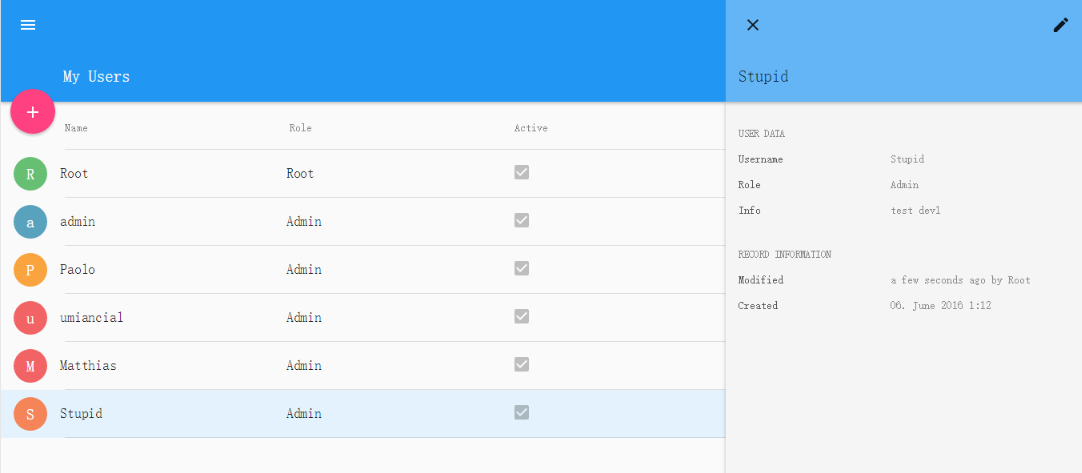
\includegraphics[width=\textwidth]{user_detail.png}
 \bicaption[fig:user_detail]{用户单个查看页面}{用户单个查看页面}{Fig}{Detail page of User}
\end{figure}
\begin{figure}[H]
 \centering
 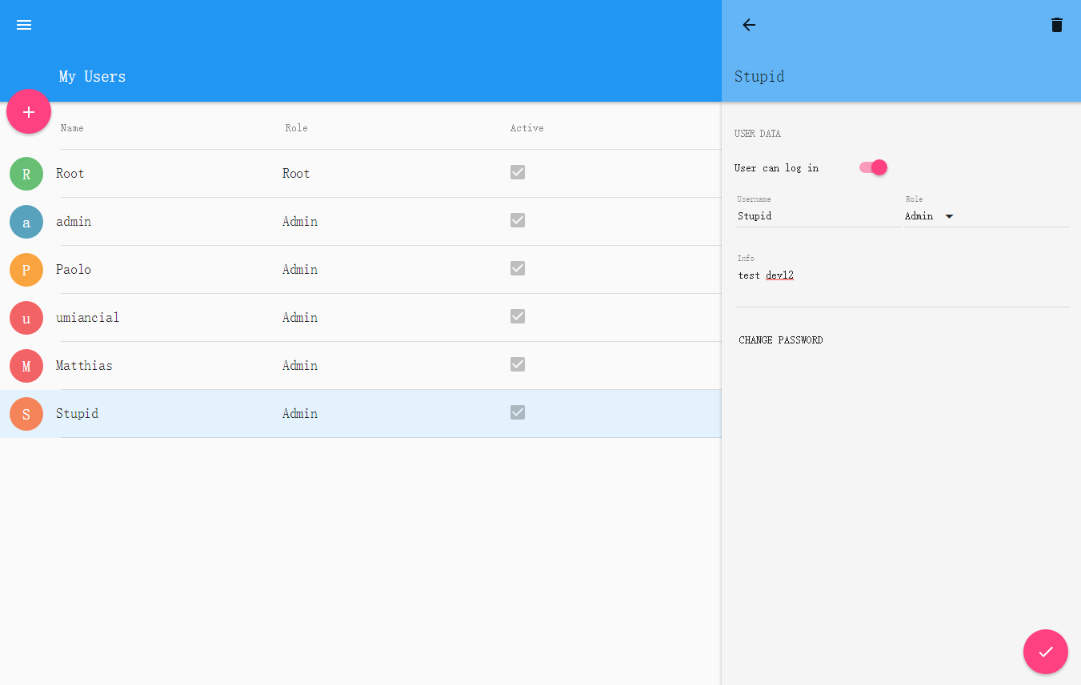
\includegraphics[width=\textwidth]{user_edit.png}
 \bicaption[fig:user_edit]{用户修改页面}{用户修改页面}{Fig}{Edit page of User}
\end{figure}
\begin{figure}[H]
 \centering
 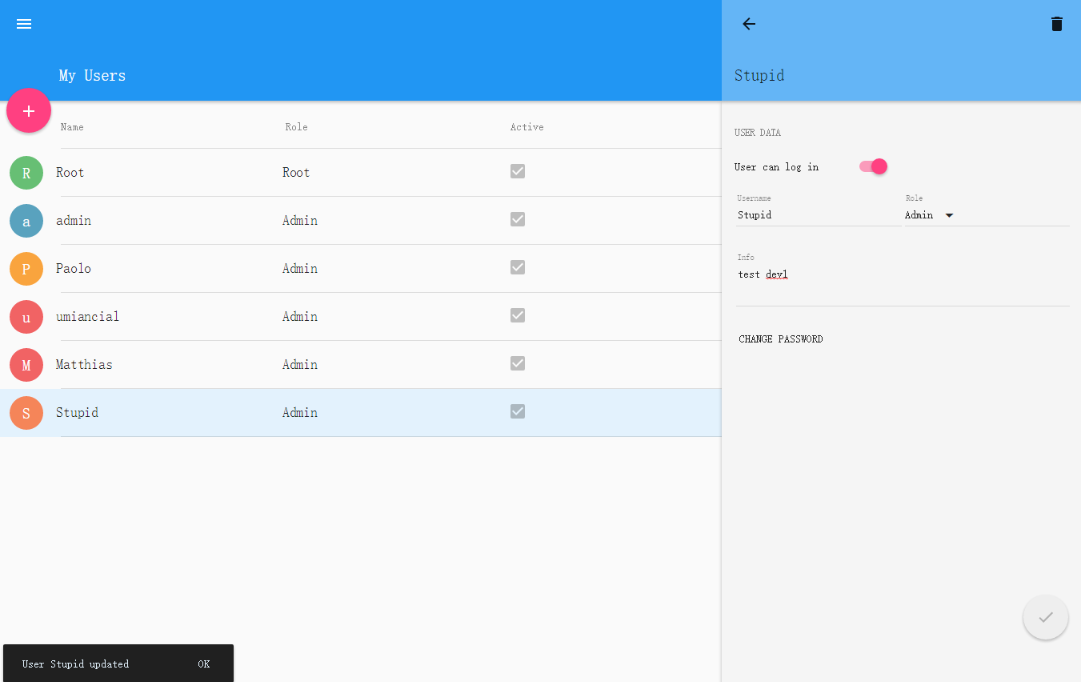
\includegraphics[width=\textwidth]{user_toastr.png}
 \bicaption[fig:user_toastr]{用户提示改动页面}{用户提示改动页面}{Fig}{Toastr box of User}
\end{figure}

\subsection{客户端模型定义}
受Mongoose的基于描述的模型(schema-based model)启发,本模块独创性地自定义了一种客户端模型定义(Client Model Definition),并开发了模型定义服务(ModelDefinitions)和与之配套使用的(当然也可以不使用)两种可重用组件(Angular中的directive)模型输入群组(ModelInputGroup)与模型视图群组(ModelViewGroup)来生成表单、列表和详情页面。

\subsubsection{模型定义服务}
模型定义服务是一个Angular服务(factory),名叫ModelDefinitions。它是一个JavaScript对象函数\footnote{JavaScript中函数也是对象,可以像对象一样拥有属性},作为函数它能够把嵌套的、带有各种简写和别称的模型定义转化为一组扁平化的属性定义(flatten PropDefinitions),如下文中代码4-2里嵌套的calibrations.mass字段会变成一个名叫'calibrations.mass'的属性定义,一个资源的模型定义最终表现形式就是属性定义数组。为方便使用扁平化的名字对模型进行操作,作为对象的模型定义服务还提供有深度扩展(deepExtend)、深度读写(deepGet和deepSet)、深度显示(deepDisplay)等辅助函数,分别是它的属性extend、get、set和display。

对于模型定义的设计,首先模仿了Mongoose模型的类型(type)、必要(required)、引用(ref)三种选项,其中引用在前端定义中是一种资源,所以叫resource。type也有比较大的差异,主要是Mongoose中的基础类型对应地变成了前端input输入框中允许的类型以及特殊的选择类型,
\begin{description}
  \item[input支持的类型] 如text(String)、url(String)、number(Number)、date(Date)、password(String),括号中为对应的Mongoose字段类型;
  \item[select] 因为JavaScript数组是弱类型的,所以select可以对应Mongoose字段的任意类型,具体类型由选项数组中的值的类型来定;
  \item[select/resource] 对应Mongoose中的ObjectId类型,和ref一样另有resource来指定资源。
\end{description}

客户端模型的每个字段除了有与Mongoose类似的类型、必要和资源三个选项外,还有一些用于定义表单输入和页面视图的选项:
\begin{description}
  \item[desc] 字符串,用于显示在输入群组和视图群组中对字段的描述,如果不填,默认为字段名的首字母大写;
  \item[displayKey] 字符串,用于显示在输入群组和视图群组中字段的值,如果字段值为对象,只显示对象中的这个指定字段;
  \item[format] 对象或正则表达式,用于输入群组中的正则格式校验,可以包含正则表达式(value)和出错信息(error)两个选项,也可使用默认出错信息直接缩写为正则表达式;
  \item[remoteUnique] 字符串,字段唯一,值为指定的资源名称,会自动检查此字段有无其他记录含有相同值;
  \item[repeatInput] 字符串,强制重复输入,值为需要重复的字段名,一般与type=password配合使用,用于重复输入密码;
  \item[validators] 对象,用于输入群组中的各类校验,上述required、format、remoteUnique和repeatInput都属于validators中配置项的简写或别号(alias),对应required、pattern、remote-unique和repeat-input;
  \item[displayPriority] 字符串,用于响应式布局的视图群组中决定是否显示字段,具体细节在下面的\textbf{响应式设计}中介绍;
\end{description}

当type为select时,表单中这个字段对应的输入组件不再是普通的输入框(input box)而是下拉列表(dropdown list),上述都是一些通用的选项,还有一些只在下拉列表中起作用的选项:
\begin{description}
  \item[options] 数组,显示在下拉列表中的选项,与displayKey和valueKey配合使用可以做到显示和实际选择的值不同;
  \item[valueKey] 字符串,实际值字段,如果选项是对象,选项在下拉列表中被选中时字段实际被赋予的值;
  \item[getOptions] 函数,异步获取选项,只在下拉列表(dropdown list)被点开时才异步地获取选项;
  \item[resource] 服务对象(service),当资源被指定时,会自动生成getOptions选项,并使用服务对象异步调用查询函数来获取选项数组;
  \item[params] 对象,在使用resource自动生成getOptions选项时,传入查询函数的参数,用于类条件查询;
\end{description}

比如对应上文传感器(Sensor)的Mongoose数据模型,由客户端模型定义的模型如代码4-4所示:
\begin{lstlisting}[language={JavaScript}, caption={Sensor的客户端模型}]
function SensorDefinition (ModelDefinitions, HardwareVersion, FirmwareVersion, ComponentBatch, ComponentTypes) {
    return ModelDefinitions({
      name: {type: 'text', required: true, remoteUnique: 'Sensor', desc: 'ID'},
      hardwareVersion: {
        type: 'select/resource',
        resource: HardwareVersion,
        desc: 'Hardware Version'
      },
      firmwareVersion: {
        type: 'select/resource',
        resource: FirmwareVersion,
        desc: 'Firmware Version'
      },
      componentBatches: {
        body: {
          type: 'select/resource',
          resource: ComponentBatch,
          params: {
            type: ComponentTypes.BODY
          },
          desc: 'Body Batch',
          displayPriority: 'low'
        },
        pcb: {
          type: 'select/resource',
          resource: ComponentBatch,
          params: {
            type: ComponentTypes.PCB
          },
          desc: 'Pcb Batch',
          displayPriority: 'low'
        },
        photodiode: {
          type: 'select/resource',
          resource: ComponentBatch,
          params: {
            type: ComponentTypes.PHOTODIODE
          },
          desc: 'PD Batch',
          displayPriority: 'low'
        },
        laser: {
          type: 'select/resource',
          resource: ComponentBatch,
          params: {
            type: ComponentTypes.LASER
          },
          desc: 'Laser Batch',
          displayPriority: 'low'
        },
        fan: {
          type: 'select/resource',
          resource: ComponentBatch,
          params: {
            type: ComponentTypes.FAN
          },
          desc: 'Fan Batch',
          displayPriority: 'low'
        }
      },
      threshold: {type: 'number', required: true},
      noiseLevel: {
        type: 'number',
        required: true,
        desc: 'Noise Level'
      },
      calibrations: {
        mass: {type: 'number', desc: 'Mass Calibration'},
        number: {type: 'number', desc: 'Number Calibration'}
      }
    });
  }
\end{lstlisting}

\subsubsection{模型输入群组}
模型输入群组(ModelInputGroup)是一个本模块开发的Angular可重用组件(directive),它包含一个模型输入组件(ModelInput),它接收一个Angular模型(ng-model,在组件内部命名为嵌套模型,nestedModel)、一组域定义(fieldDefinitions,因为在表单中所以命名为域定义而不是属性定义)和一个表单对象(form)。模型输入群组会把域定义数组中的每个域定义再传递给模型输入组件。因为域定义是扁平化的,直接按照域定义很难直接管理实际需要的嵌套模型,所以模型输入群组内部额外维护了一个的扁平模型,用户在模型输入组件中输入时直接更新的是扁平模型,然后使用模型定义服务的深度赋值函数对嵌套模型进行修改。如代码4-3所示,只需要插入这样一段调用组件的HTML代码,就可以在传感器资源的创建(create)页面渲染出如图4-1所示的一组输入组件,在修改(edit)页面上也类似。
\begin{lstlisting}[language={HTML5}, caption={传感器创建页面中的模型输入群组代码}]
<model-input-group ng-model="create.sensor"
                   form="createForm"
                   field-definitions="create.sensorDefinition">
</model-input-group>
\end{lstlisting}
\begin{figure}[H]
 \centering
 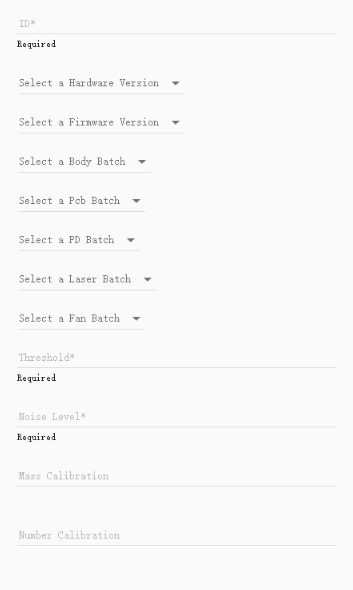
\includegraphics[width=0.6\textwidth]{sensor_create.png}
 \bicaption[fig:sensor_create]{传感器创建页面表单}{传感器创建页面表单}{Fig}{Form in create page of Sensor}
\end{figure}
\subsubsection{模型视图群组}
模型视图群组(ModelViewGroup)也是一个本模块开发的Angular可重用组件,它接收一个模型对象(model,这里不需要修改所以不需要用ng-model)、一组属性定义和一个类型。还有可选项狭窄模式(narrow-mode),用于响应式布局。类型可以分为:
\begin{enumerate}
  \item items-header(列表头部,只横向列出每个属性定义的描述,此类型不需要传入模型对象)
  \item items-content(列表内容,使用模型定义服务的深度显示函数横向列出模型对象每个属性定义的数值)
  \item detail(详细内容,竖向列出属性定义的描述和对应的数值)
\end{enumerate}
如代码4-4所示,只需要插入这样几段调用组件的HTML代码,并且当前app打开了细节页面时(app.inDetailState为true),就可以在传感器资源的列表(list)和细节(detail)页面渲染出如图4-2所示的一组视图组件。
\begin{lstlisting}[language={HTML5}, caption={传感器列表页面中的模型输入群组代码}]
<!-- in items.html -->
<model-view-group definitions="index.sensorDefinition"
                  type="items-header"
                  narrow-mode="app.inDetailState">
</model-view-group>
...
<model-view-group model="sensor"
                  definitions="index.sensorDefinition"
                  type="items-content"
                  narrow-mode="app.inDetailState">
</model-view-group>
<!-- in detail.html -->
<model-view-group model="detail.sensor"
                  definitions="index.sensorDefinition"
                  type="detail">
</model-view-group>
\end{lstlisting}
\begin{figure}[!htp]
 \centering
 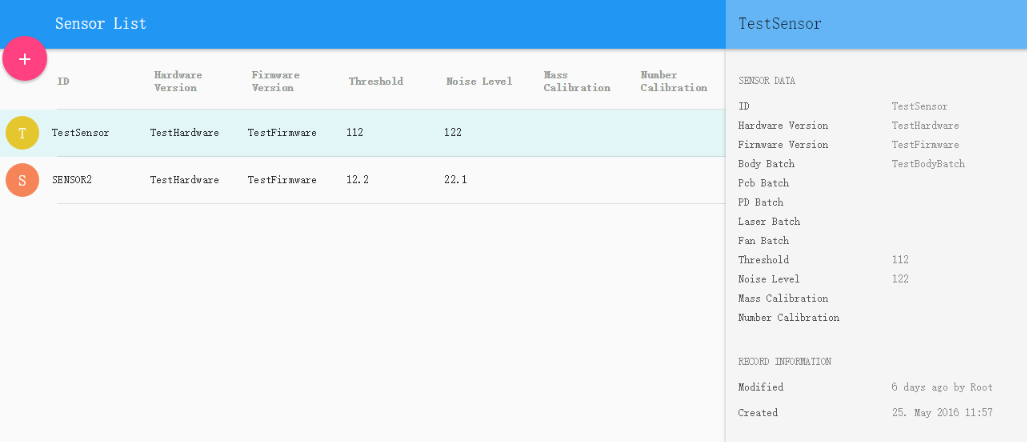
\includegraphics[width=\textwidth]{sensor_detail.png}
 \bicaption[fig:sensor_detail]{传感器细节页面}{传感器细节页面}{Fig}{Detail page of Sensor}
\end{figure}
\subsection{响应式设计}


\subsection{代码生成器}
\subsection{Git提交记录}
\section{Smart Home 和 Smart City模块}
\subsection{前端}
\subsubsection{redux管理数据流}
\subsubsection{Echarts绘制图表}
\subsection{后端和数据库}
\subsubsection{socket-io实时更新}
\section{主要组件详细设计}
\subsection{客户端ORM表单组件}
\subsection{EChart组件}
\subsection{AqiChart组件}
\subsection{AqiMap组件}
\subsection{API组件}
